\documentclass[12pt]{article}
\usepackage[margin=0.7in]{geometry} 		% defines page margin
\usepackage{knitting} 				% defines \chart and \textknit
\usepackage{titling} 				% title page
\usepackage{graphicx,xspace, scrextend}	% defines space control stuff
\usepackage{tabularx, array, colortbl}	% defines tables
\usepackage{multicol} 				% defines columns
\usepackage{multirow} 				% defines multirows, combined cells in tables
\usepackage{framed} 				% defines boxes for notes and written directions
\usepackage[x11names]{xcolor} 		% extends color library
\usepackage{hyperref}				% hyperlinks
\usepackage{wrapfig}
\hypersetup{
    colorlinks=true,
    linkcolor=blue,
    filecolor=magenta,      
    urlcolor=blue,
}

\pdfmapfile{+knitfont.map}

% font selection
\usepackage{palatino, moresize, sectsty}
\allsectionsfont{\sffamily}

% PICK AND CHOOSE COMMANDS BASED ON NEEDS

\renewcommand{\arraystretch}{1.5} % compresses tables for pattern keys

\newcolumntype{L}[1]{>{\leftalign\arraybackslash}p{#1}}
\newcolumntype{C}[1]{>{\centering\arraybackslash}p{#1}}

% length parameters
\setlength{\parindent}{0pt} % disables indentation for paragraphs
\setlength{\columnsep}{0.7cm} % column separation in multicol environment

% color parameters
\colorlet{framecolor}{black}
\colorlet{shadecolor}{LemonChiffon1}
\colorlet{highlight}{yellow}

% custom commands
\newcommand{\comment}[1]{} % allows for multiline comments that LaTeX will ignore

\newcommand{\vocab}[1]{\emph{\textbf{#1}}} % format for highlighting definitions of stitches, vocabulary terms
\newcommand{\rowDir}[1]{\textbf{#1:}} % indent for written instructions within paragraphs

\renewcommand{\repeat}[1]{\textbf{[#1]}} % format for written repeats, bold with *[ stitches ]*
\newcommand{\repmark}{\textbf{*}}
\newcommand{\longrepeat}[1]{\textbf{\repmark} #1, repeat from \repmark}%\textbf{*}}
\newcommand{\x}{$\times$}			% times symbol but shorthand
\newcommand{\setrepeat}[2]{\textbf{[#1]}\x{#2}}		% format for repeats with set number of repetitions, bold with [ stitches ]

\newcommand{\blank}{\underline{\hspace{2em}} } % written instructions, fill-in-the-blank box
\newcommand{\highlighted}[1]{\colorbox{highlight}{#1}} % written instructions, highlight particular text


% stitch count commands
\newcommand{\increase}[1]{(\emph{+#1 
	\ifnum#1=1{st}\else{sts}\fi})}
\newcommand{\decrease}[1]{(\emph{$-$#1
	\ifnum#1=1{st}\else{sts}\fi})}
\newcommand{\stitchcount}[1]{(\emph{#1 sts})}

% marker instructions
\renewcommand{\pm}[1]{\emph{pm #1}} % place stitch marker
\newcommand{\sm}{\emph{sm}} % slip marker
\renewcommand{\rm}[1]{\emph{rm #1}} % remove stitch marker

% thick horizontal line
\makeatletter \newcommand{\thickhline}{
    \noalign {\ifnum 0=`}\fi \hrule height 1.5pt
    \futurelet \reserved@a \@xhline
}
\makeatother

% custom environments
\newenvironment{frnote}
    {% framed environment for pattern notes
    	\setlength{\FrameRule}{1.5pt}
    	\def\FrameCommand{\fboxrule=\FrameRule\fboxsep=\FrameSep \fcolorbox{framecolor}{shadecolor}}
    	\MakeFramed {\FrameRestore}}
    {\setlength{\FrameRule}{1pt}
	\endMakeFramed}

\newenvironment{frdirection}
    {% framed environment for written directions
	\def\FrameCommand{\fboxrule=\FrameRule\fboxsep=\FrameSep \fbox}
   	\MakeFramed {\advance\hsize-\width \FrameRestore}
    	\addmargin[1.5cm]{0pt}}
    {\endaddmargin
	\endMakeFramed}

\newenvironment{unframed}
    {% unframed environment for written directions
	\begin{addmargin}[2em]{0pt}
	\setlength{\parindent}{-2em}}
    {%\vspace{1em}
	\setlength{\parindent}{0em}
	\end{addmargin}}

\title{Planetes} % pattern name here
\author{Shanel Wu (Piper Nell)}

\begin{document}

%%%%%%%%%%%%%%%%%%%%%%%%%%%%%%%%%%%%%%%%%%%%%%%%%%
% TITLE PAGE 

% COVER PHOTO
% uncommend line below if you want a background fill image
% \ThisLRCornerWallPaper{1.0}{image.jpg} 

{\fontfamily{qag}\selectfont
\HUGE\textbf{\thetitle}
\hspace{2em} \hfill % adjust this space or use \hfill
\normalsize\theauthor
}

\begin{multicols}{2}
\small

\includegraphics[width=\linewidth]{Photos/smallVersions/Planetes_R3}

% Cute description here
\vspace{1em}
$\pi\lambda\alpha\upsilon\acute{\eta}\tau\eta\varsigma$ (plan\'{e}t\={e}s) - an Ancient Greek word meaning ``to wander". Planets like Venus, Mars, Mercury, and Jupiter appeared to be wandering stars, finding their own path in a vast sky.

~\\
Many of my friends (including me) moved far away from our hometowns to places with harsh winters, chasing dreams, passions, and callings. I love making slippers for loved ones in these situations to help them feel at home wherever they are. I designed these slippers to warm anyone’s feet and add a pop of colorful cheer.

~\\
\vfill
~\\
\columnbreak

\subsection*{Sizing: XS (S, M, L, XL)}

Fits EU shoe sizes 18-24 (25-32, 33-43, 44-49, 50+) or baby (child/adult narrow, adult medium, adult wide, adult XL/felting). Sizes correspond to foot widths of 2.5 (3.5, 4.5, 5.5, 6.5)" / 6.5 (9, 11.5, 14, 16.5) cm. Each size is written with a default foot length, which can be adjusted by following the instructions on the following page. Select size based on foot width.


\subsection*{Yarn Requirements}

% yardage, number of colors, etc.
DK weight yarn held double, or aran/bulky weight alone, in three colors (C1, C2, C3).

{\fontsize{10pt}{12} \selectfont

\rowDir{C1} 25 (60, 120, 190, 260) yds / 25 (55, 110, 170, 240) m

\rowDir{C2} 15 (30, 40, 50, 70) yds / 15 (30, 40, 50, 70) m

\rowDir{C3} 30 (75, 150, 230, 330) yds / 30 (70, 140, 220, 300) m
}

% also include: sample yarn, other yarn suggestions
{\scriptsize
\emph{Sample: Rauma 3tr Strikkegarn (118yds/50g, 100\% Norwegian wool) in \\C1 - 1387 (navy blue), C2 - 146 (yellow), C3 - 138 (light blue).}
}


\subsection*{Gauge: 16 sts x 24 rows = 4"/10cm}

% sample measurements, gauge, notes on ease, etc.
or 4 sts x 6 rows = 1"/2.5cm. Gauge is measured over slightly stretched stockinette stitch. A dense fabric is necessary for long-wearing socks. If you obtain a gauge tighter than 4 sts/1", choose a larger size sock instead of switching needle sizes.

\subsection*{Tools}

\begin{itemize}
\item \rowDir{Size A} US7/4.5mm (or size needed to obtain tight gauge) in any style % NEEDLES
\item \rowDir{Size B} US9 (or 2 sizes larger than Needle A to work cuff)
\item crochet hook and scrap yarn
\item stitch markers% STITCH MARKERS
\end{itemize}

\subsection*{Techniques}

This pattern is suitable for an intermediate knitter. % DIFFICULTY LEVEL
Prior to knitting this pattern, you should be familiar with provisional cast ons, increases, decreases, and simple cables. % PREREQUISITE TECHNIQUES
For a complete list of stitches used, see Pattern Key.

~\\
% discuss any special techniques and tutorials included

\vfill
\newpage
%%%%%%%%%%%%%%%%%%%%%%%%%%%%%%%%%%%%%%%%%%%%%%%%%%
% FOREWORD

\subsection*{Pattern Key}

% abbreviation key - fill in with all abbreviations/stitch patterns used in design: written abbreviation, full stitch name or explanation
% try to keep them in sequential order as they appear in the pattern, or in an order that builds upon previous definitions
% chart symbols included in separate keys attached to their respective charts
% stitches with explanations must first be BOLDED, followed by colon then explanation

\vocab{Written instructions:} repeats = \repeat{stitches} or \\\longrepeat{thing to do}

\vspace{-1em}
\begin{center}
{\renewcommand{\arraystretch}{1.2}
\begin{tabular}{| C{0.2\linewidth}  p{0.6\linewidth} | }
\thickhline \rowcolor{shadecolor} 
\textbf{Abbr.}	& \textbf{Description} \\ \thickhline
CO 	& cast on \\
BO 	& bind off \\
RS 	& right side \\
WS 	& wrong side \\
pm	& place stitch marker \\
sm	& slip stitch marker \\
k	&  knit \\
p	& purl   \\
k2tog 	& knit 2 together \\
p2tog	& purl 2 together \\
ssk	& slip slip knit \\
sl 	& slip st (stitch) purlwise \\ 
sl1 wyib & sl 1 st with yarn in back \\
sl1 wyif & sl 1 st with yarn in front \\
psso 	& pass slipped st over \\
kfb 	& knit front back \\
C4B 	& slip 2 sts to cable needle and hold at back, k2, k2 sts from cable needle \\
C4F 	& slip 2 sts to cable needle and hold at front, k2, k2 sts from cable needle \\
\hline
\end{tabular}
}
\end{center}

~\\
\vfill
\columnbreak
\section*{Construction}

The slipper begins with the back of the leg, proceeds down around the heel and sole, bends around the toe, then travels up the instep with a decorative cable pattern. The slipper finishes with a Latvian braid cuff. Each colored section in the schematic corresponds to a numbered section in the instructions.

\vspace{-1em}
\begin{center}
\includegraphics[width=.9\linewidth]{Planetes_schematic.png}
\end{center}

%\begin{addmargin}[-2em]{0em}
{\fontsize{10pt}{12} \selectfont
{\small\textbf{\textsf{A: Foot Width}}} \\\hspace{.2em} 2.5 (3.5, 4.5, 5.5, 6.5)" / 6.5 (9, 11.5, 14, 16.5) cm \\

{\small\textbf{\textsf{B: Leg Height}}} \hspace{.5em} 2 (3, 5, 6, 7)" / 5 (7.5, 12.5, 15, 17.5) cm \\

{\small\textbf{\textsf{C: Foot Length}}} \\\hspace{.5em} 4 (7, 9, 11, 13)" / 10 (17.5, 22.5, 27.5, 32.5) cm \\
}


%\end{addmargin}
\end{multicols}

\begin{wrapfigure}{R}{0.7\linewidth}
\includegraphics[width=0.8\linewidth]{Planetes_chart.png} \hspace{1.5in}
\vspace{-1in}
\end{wrapfigure} \leavevmode

\vspace{-3em}
\subsection*{Cable Pattern}

\rowDir{Row 1 (RS)} k8

\rowDir{Row 2 (WS)} k2, p4, k2

\rowDir{Row 3} k8

\rowDir{Row 4} p8

\rowDir{Row 5} C4B, C4F

\rowDir{Row 6} p8

\normalsize
\newpage

%%%%%%%%%%%%%%%%%%%%%%%%%%%%%%%%%%%%%%%%%%%%%%%%%%
% BEGIN INSTRUCTIONS
\section*{1. Back Leg}

Using a crochet hook and scrap yarn (or preferred method), provisionally CO 10 (14, 18, 22, 26) sts 
using C1. The first row worked into the CO is a RS row.

\rowDir{Row 1} Sl1 wyif, k to end.

Repeat Row 1 on both RS and WS (garter st) until piece measures 2 (3, 5, 6, 7)" / 5 (7.5, 12.5, 15, 17.5) cm or until desired leg height, ending after a WS row.

\begin{wrapfigure}{R}{0.25\linewidth}
\vspace{1em}
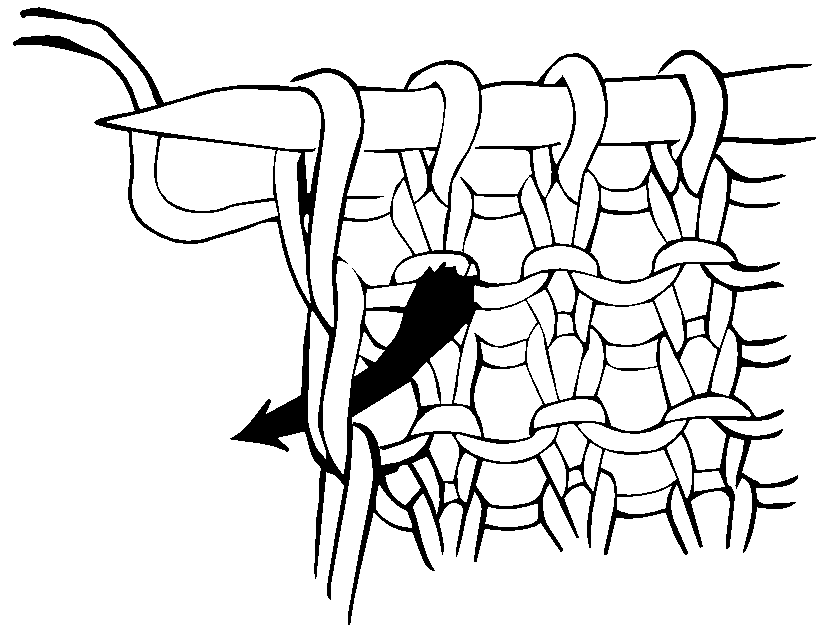
\includegraphics[width=\linewidth]{punk.png}
\emph{\small \textbf{A:} Insert R needle in this direction to pick up and knit in selvedge.}

\vspace{2em}
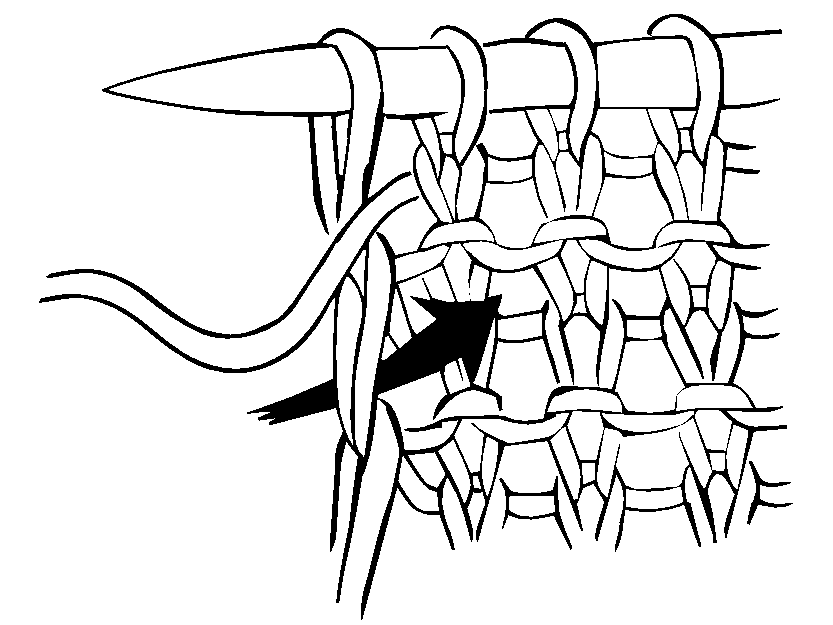
\includegraphics[width=\linewidth]{punp.png}
\emph{\small \textbf{B:} Insert R needle in this direction to pick up and purl in selvedge.}
\vspace{-5em}
\end{wrapfigure} \leavevmode

\section*{2. Heel}

\subsection*{Part A}

Change to C2. You can actually join C2 without cutting C1, to pick it up later. Repeat Row 1 6 (8, 8, 10, 12) more times. Then, work Row 2 a total of 6 (8, 12, 14, 18) times until 4 (6, 6, 8, 8) sts remain.

\rowDir{Row 2} Sl1 wyif, k to 3sts from end, k2tog, k1.

\subsection*{Part B}

Work Rows 3 and 4 once to set up the second part of the heel.

\rowDir{Row 3 (RS)}  sl1 wyib, k to 2 sts from end, kfb, sl1 wyib, pick up and knit first selvedge st below (see diagram \vocab{A}), psso and turn.

\rowDir{Row 4 (WS)} sl1 wyif, k to 2 sts from end, kfb, sl1 wyif, pick up and purl first selvedge st below (see diagram \vocab{B}), psso and turn.

~\\
Then, repeat Rows 5 and 6 a total of 4 (6, 8, 10, 12) times until you have worked a st in all C2 selvedge sts. 14 (20, 24, 30, 36) total sts.

\rowDir{Row 5 (RS)} sl1 wyib, k to 2 sts from end, kfb, sl1 wyib, pick up and knit 1 st in selvedge, psso and turn.

\rowDir{Row 6 (WS)} sl1 wyif, k to 2 sts from end, kfb, sl1 wyif, pick up and purl 1 st in selvedge, psso and turn.

\section*{3. Sole with Gusset}

Change back to C1. Work Rows 7 and 8 a total of 2 (3, 3, 4, 5) times until you return to 10 (14, 18, 22, 26) % original CO num
total sts.

\rowDir{Row 7 (RS)} sl1 wyib, k to 3 sts from end, ssk, k1.

\rowDir{Row 8 (WS)}  sl1 wyif, p to 3 sts from end, p2tog, p1. 

~\\
Work Rows 9 and 10 approximately 5 (10, 16, 21, 25) total times until piece measures 3 (5.5, 7.5, 9.5, 11.5)" / 7.5 (13.75, 18.75, 23.75) cm from the heel, or until 1 (1.5, 1.5, 1.5)" / 2.5 (3.75, 3.75, 3.75) cm short of the toe.

\rowDir{Row 9 (RS)} sl1 wyib, k to end.

\rowDir{Row 10 (WS)} sl1 wyif, p to end.

\begin{wrapfigure}{R}{0.32\linewidth}
\vspace{3em}
\includegraphics{Photos/smallVersions/Planetes_toe} \hspace{1em}
\vspace{-6em}
\end{wrapfigure} \leavevmode

\section*{4. Toe}

The toe is nearly identical to the heel, except that you're working with fewer stitches.

\subsection*{Part A}
Break C1 and change to C2. Work Row 2 a total of 6 (10, 12, 14, 18) times until 4 (4, 6, 8, 8) sts remain, ending after a WS row.

\rowDir{Row 2} Sl1 wyif, k to 3sts from end, k2tog, k1.

\subsection*{Part B}
Work Rows 3 and 4 once to set up the second part of the toe.

\rowDir{Row 3 (RS)}  sl1 wyib, k to 2 sts from end, kfb, sl1 wyib, pick up and knit first selvedge st below (see diagram \vocab{A}), psso and turn.

\rowDir{Row 4 (WS)} sl1 wyif, k to 2 sts from end, kfb, sl1 wyif, pick up and purl first selvedge st below (see diagram \vocab{B}), psso and turn.

~\\
Then, repeat Rows 5 and 6 a total of 2 (4, 5, 6, 8) times to return to 10 (14, 18, 22, 26) total sts.

\rowDir{Row 5 (RS)} sl1 wyib, k to 2 sts from end, kfb, sl1 wyib, pick up and knit 1 st in selvedge, psso and turn.

\rowDir{Row 6 (WS)} sl1 wyif, k to 2 sts from end, kfb, sl1 wyif, pick up and purl 1 st in selvedge, psso and turn.

\section*{5. Instep}

Break C2 and change to C3. Work Rows 11 and 12 once to set up the instep pattern. For size XS, note that there are no sts between the selvedge st and marker. 

\rowDir{Row 11 (RS)} sl1 wyib, k - (2, 4, 6, 8), pm, work Row 1 of Cable Chart, pm, k - (2, 4, 6, 8), sl1 wyib, pick up and knit 1 st in selvedge, psso and turn.

\rowDir{Row 12 (WS)} sl1 wyif, k - (2, 4, 6, 8), sm, work Row 2 of Cable Chart, sm, k - (2, 4, 6, 8), sl1 wyif, pick up and purl 1 st in selvedge, psso and turn.

~\\
Then, repeat Rows 13 and 14, working through the Cable Chart, until you have 1-3 selvedge sts left unworked after completing Row 6 of the chart. 

\rowDir{Row 11 (RS)} sl1 wyib, k - (2, 4, 6, 8), sm, work next row of Cable Chart, sm, k - (2, 4, 6, 8), sl1 wyib, pick up and knit 1 st in selvedge, psso and turn.

\rowDir{Row 12 (WS)} sl1 wyif, k - (2, 4, 6, 8), sm, work next row of Cable Chart, sm, k - (2, 4, 6, 8), sl1 wyif, pick up and purl 1 st in selvedge, psso and turn.

~\\
To finish instep, repeat Rows 13 and 14 but instead of cable pattern, work garter st (i.e. k all sts between markers) until all selvedge sts have been worked.

\section*{6. Cuff}

\rowDir{Next row (RS)} sl1 wyib, k to end, removing all markers as they come. Instead of turning work, unpick provisional CO and k all live sts. You may have to use the CO tail to secure the last st. Join in the round and pm for end of the round. 20 (28, 36, 44, 52) total sts.

\begin{wrapfigure}{L}{0.4\linewidth}
\vspace{-0em}
\includegraphics[width=\linewidth]{Photos/smallVersions/Planetes_cuff2}
\end{wrapfigure}\leavevmode

Switch to larger needles. Join C3 and work Latvian braid as follows using both C2 and C3.

\rowDir{Rnd 1} \repeat{k1 C2, k1 C3} around. Carry the strand not in use on the WS.

\rowDir{Rnd 2} Bring both yarns forward to RS. \longrepeat{p1 C2, bring C3 \emph{under} C2 to twist yarns, p1 C3, bring C2 \emph{under} C3 to twist} around.

\rowDir{Rnd 3} \longrepeat{p1 C2, bring C3 \emph{over} C2 to twist in opposite direction, p1 C3, bring C3 \emph{over} C2} around.

These instructions produce a right-leaning braid. For a left-leaning braid, switch Rnds 2 and 3 (i.e. twist \emph{over} first, and then \emph{under}).

~\\
Break C2. BO loosely and/or with a stretchy method using C3. Weave in all ends. Repeat for second sock, and block or felt if desired.

%%%%%%%%%%%%%%%%%%%%%%%%%%%%%%%%%%%%%%%%%%%%%%%%%%
% APPENDICES (IF ANY)
\section*{Modification Suggestions}
\subsection*{Adjusting Length/Height}

\begin{tabular}{p{0.2\linewidth} p{0.8\linewidth}}
\textbf{Foot Length: \blank} &  Measure your foot from heel to toe to determine the foot length of your socks. \\

\textbf{Leg Height: \blank} & For a \emph{long} sock as shown in the sample, divide the foot length by 2. For a short sock, divide the foot length by 3 or by 4. \\
\end{tabular}

\subsection*{Adjusting Width}
Adjusting width will be a more extensive modification. If none of the written sizes suits your needs (maybe you're modifying for a different gauge or more/less ease), you can CO any even number of stitches to obtain your desired width. At the heel, work \textbf{Row 2} an even number of times until you decrease to approximately a half of your CO sts. In the second half of the heel, repeat \textbf{Rows 5 and 6} until you've increased by a third of the CO stitch count. Repeat \textbf{Rows 7 and 8} until you return to the CO stitch count. At the toe, work \textbf{Row 2} an even number of times until you decrease to approximately half of your CO sts. Increase back to the original CO stitch count to complete the instep.

%%%%%%%%%%%%%%%%%%%%%%%%%%%%%%%%%%%%%%%%%%%%%%%%%%
% COPYRIGHT

\begin{frnote} \ssmall
Pattern and photographs \copyright 2019 Shanel Wu.
All rights reserved. In purchasing this pattern, you agree to print and use this pattern only for personal use. Do not redistribute or sell paper or electronic copies of this pattern.
\end{frnote}

\end{document}